%!TEX root = main_RNAPyro_JCB.tex
\section{Results}
\label{sec:results}

\subsection{Implementation}
The software was implemented in Python2.7 using the \textit{mpmath}~\cite{mpmath} library
for  arbitrary floating point precision. The source code is freely available at:

%{\centering \url{https://github.com/McGill-CSB/RNApyro}\\}
%\TODOJerome{Did we set up an ad hoc website?}

{\centering \url{http://csb.cs.mcgill.ca/RNApyro}\\}
The time benchmarks were performed on an AMD Opteron(tm) Processor 6278  at 2.4 GHz with cache of 512 KB.20 cores and 175 GB ram.
Since typical use-cases of \RNApyro require efficiency and scalability, we present in TableFigure~\ref{fig:time}
typical runtimes required to compute the probabilities for  every nucleotide at every positions for a vast set of parameters.
For those tests, both the multiple sequence alignment and the reference sequence were generated uniformly at random,
based on a realistic random secondary structure, generated as described in Levin~\emph{et al}~\cite{Levin:2012kx}.
\TODOVlad{Add more extensive time benchmark, as a plot}
%\TODOVlad{Is time benchmark still on Mac mini or mcbbigram?}

\begin{figure}[t]
{\centering 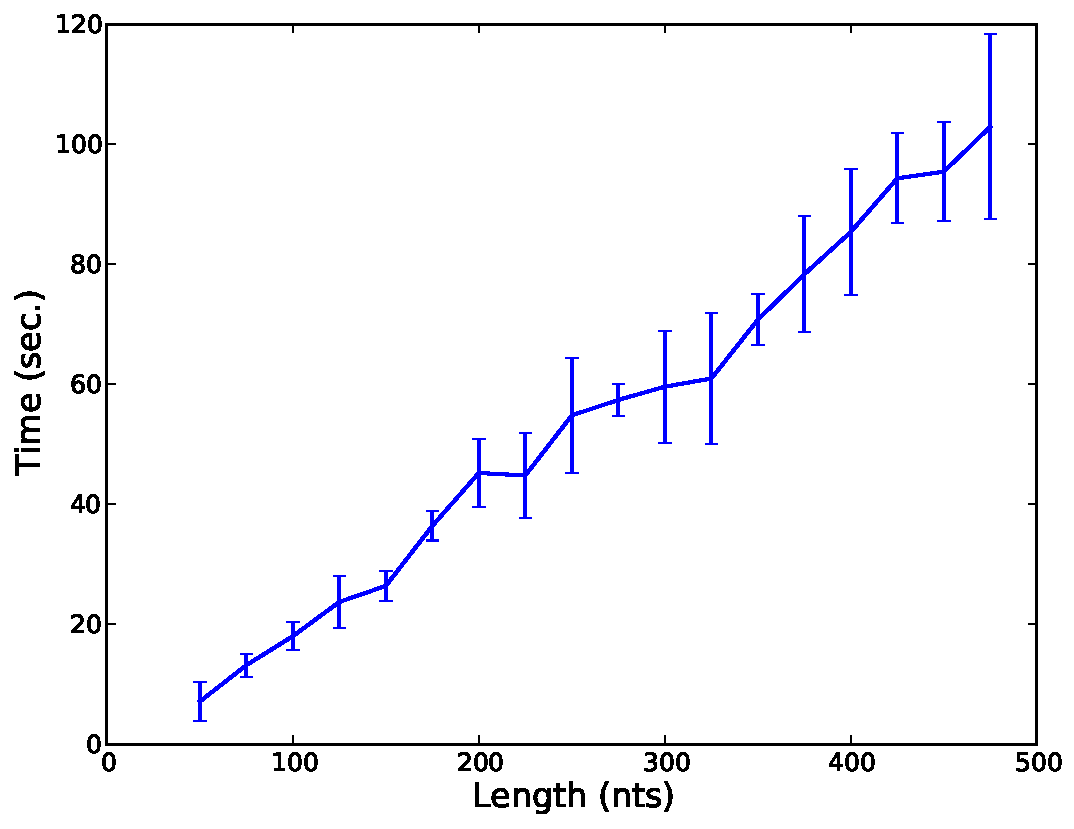
\includegraphics[width=.5\linewidth]{figures/TimeBenchmark}\\}

\caption{Typical runtimes required by the computation of mutational profiles 
averaged on $50$ random sequences for each length ranging from $100$ and $400$ nts, while allowing for a maximal number mutations equal to $M=10$. 
For each sequence, a random multiple sequence alignment was generated, consisting of $51$ aligned sequences, each compatible with a randomly generated consensus secondary structure. 
}
\label{fig:time}
\end{figure}


\subsection{Homogenous Error Correction in 5s rRNAs}
\label{sec:5S}
To illustrate the potential of our algorithm, we applied our techniques to identify and correct point-wise errors in RNA sequences
with conserved secondary structures. More precisely, we used \RNApyro to reconstruct 5s rRNA sequences with randomly distributed
mutations. This experiment has been designed to suggest further applications to error-corrections in pyrosequencing data.

We built our data set from the 5S rRNA multiple sequence alignment (MSA) available in the Rfam Database 11.0 (Rfam id: \texttt{RF00001}).
Since our software does not currently implement gaps (mainly because scoring indels is a challenging issue that cannot be fully addressed
in this work),  we clustered together the sequences with identical gap locations. From the $54$ MSAs without gap produced, we selected the
biggest MSA  which contains $130$ sequences (out of $712$ in the original Rfam MSA). Then, in order to avoid overfitting, we used \texttt{cd-hit}
\cite{Li:2006fk} to remove sequences with more than 80\% of sequence similarity. This operation resulted in a data set of $45$ sequences. 

We designed our benchmark using a leave-one-out strategy. We randomly picked a single sequence from our data set and performed $12$ random
mutations, corresponding to an error-rate of 10\%. We repeated this operation $10$ times. The value of $\beta$ was set to $15$ (larger values gave similar results). 
To estimate the impact on the distribution of the relative weights of energy and isostericity, we used 4 different values of $\alpha = {0, 0.5, 0.8, 1.0}$. 
Similarly, we also investigated the impact of an under- and over- estimate of the number of errors, by setting the presumed number of errors to 50\% (6 mutations) and 200\% (24 mutations) of their exact number (i.e. $12$).

To evaluate our method, we computed a ROC curve representing the performance of a classifier based on the mutational probabilities computed
by \RNApyro. More specifically, we fixed a threshold $\lambda \in [0,1]$, and predicted an error at position $i$ in sequence $\omega$ if and only if the
probability $P(i,x)$ of a nucleotide $x$ exceeds this threshold. To correct the errors we used the set of nucleotides having probability
greater than $\lambda$, that is  
$$C(i) = \{ x \; | \;  x \in \{ \Ab,\Cb,\Gb,\Ub \}, P(i,x) > \lambda \mbox{ and }  n \neq \omega[i] \},$$
 where $\omega[i]$ is
the nucleotide at position $i$ in the input sequence. We note that, for lower thresholds, multiple nucleotides may be available in $C(i)$ to correct
the sequence. Here, we remind that our aim is to estimate the potential of error-correction of \RNApyro, and not to develop a full-fledged error-correction pipe-line, which  
shall be the subject of further studies. Finally, we progressively varied $\lambda$ between $0$ and $1$ to calculate the ROC curve and the area
under the curve (AUC). Our results are reported in Figure~\ref{fig:ROCall}. 

\begin{figure}
\centering
	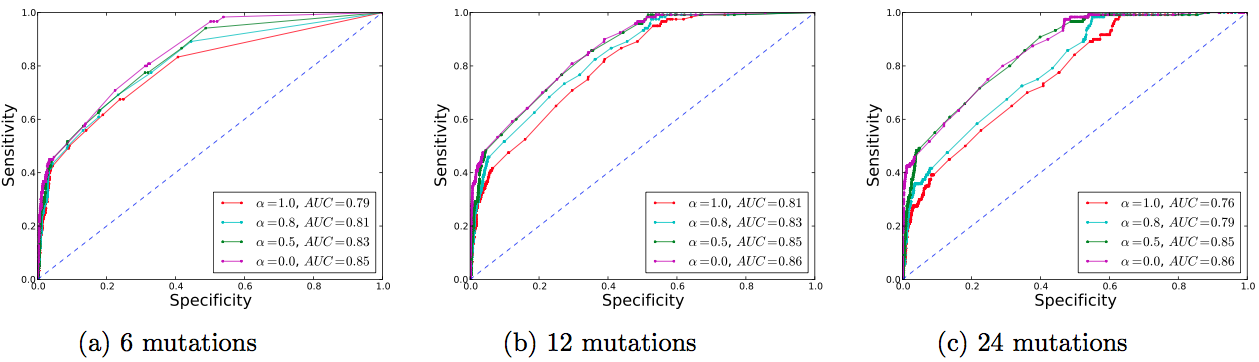
\includegraphics[width=\textwidth]{subfigs_perform.png}\\

%\begin{subfigure}[b]{0.3\textwidth}
%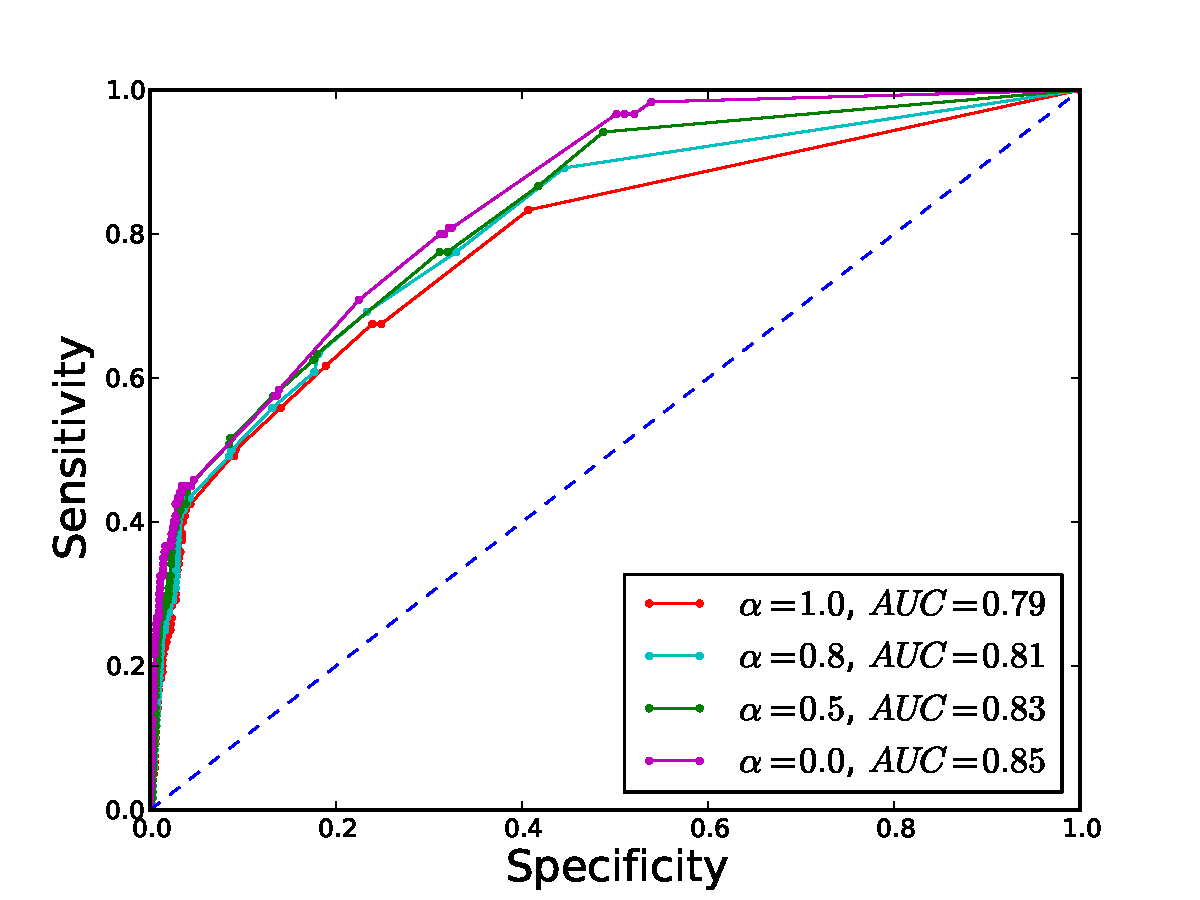
\includegraphics[width=1.2\textwidth]{figures/ROC_6.pdf}
%\caption{6 mutations}
%\label{fig:ROC6mut}
%\end{subfigure}
%\hfill
%\begin{subfigure}[b]{0.3\textwidth}
%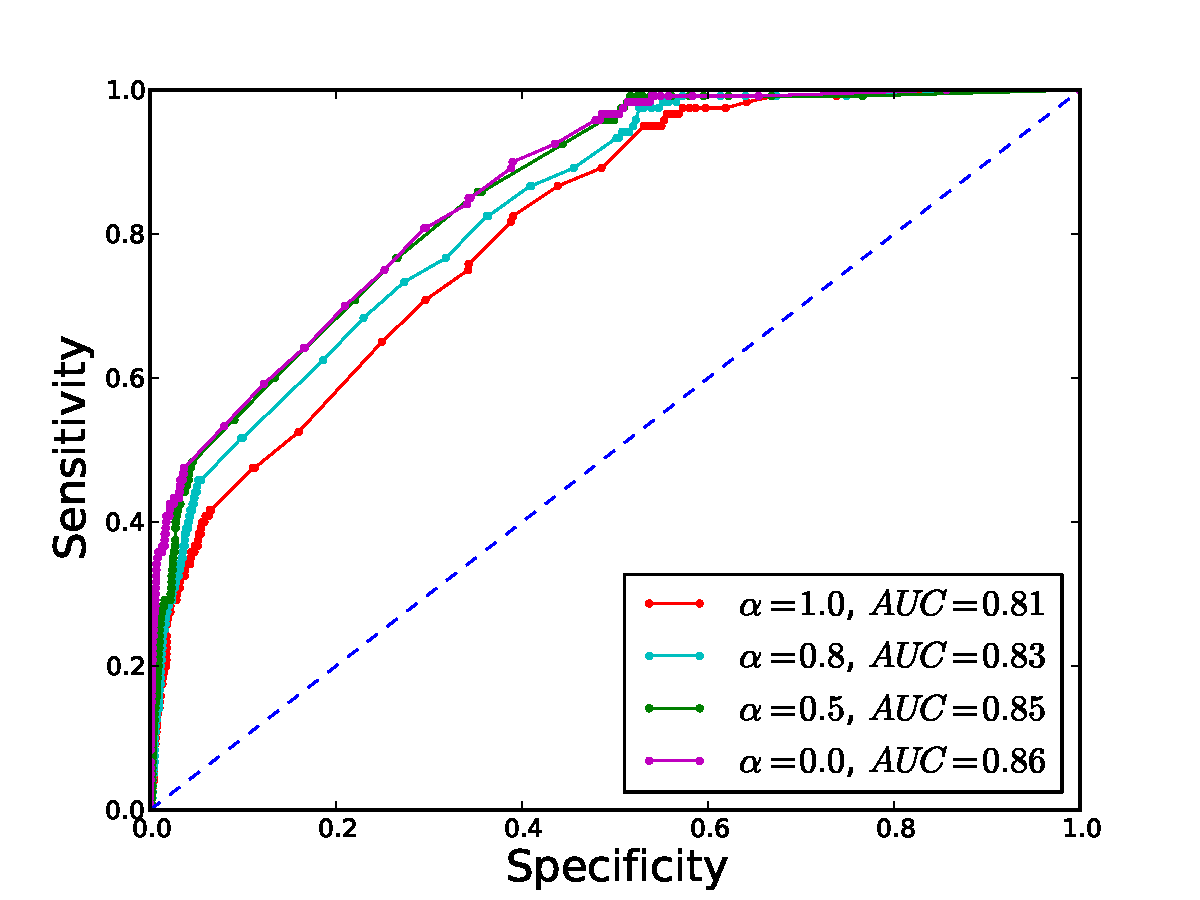
\includegraphics[width=1.2\textwidth]{figures/ROC_12.pdf}
%\caption{12 mutations}
%\label{fig:ROC12mut}
%\end{subfigure}
%\hfill
%\begin{subfigure}[b]{0.3\textwidth}
%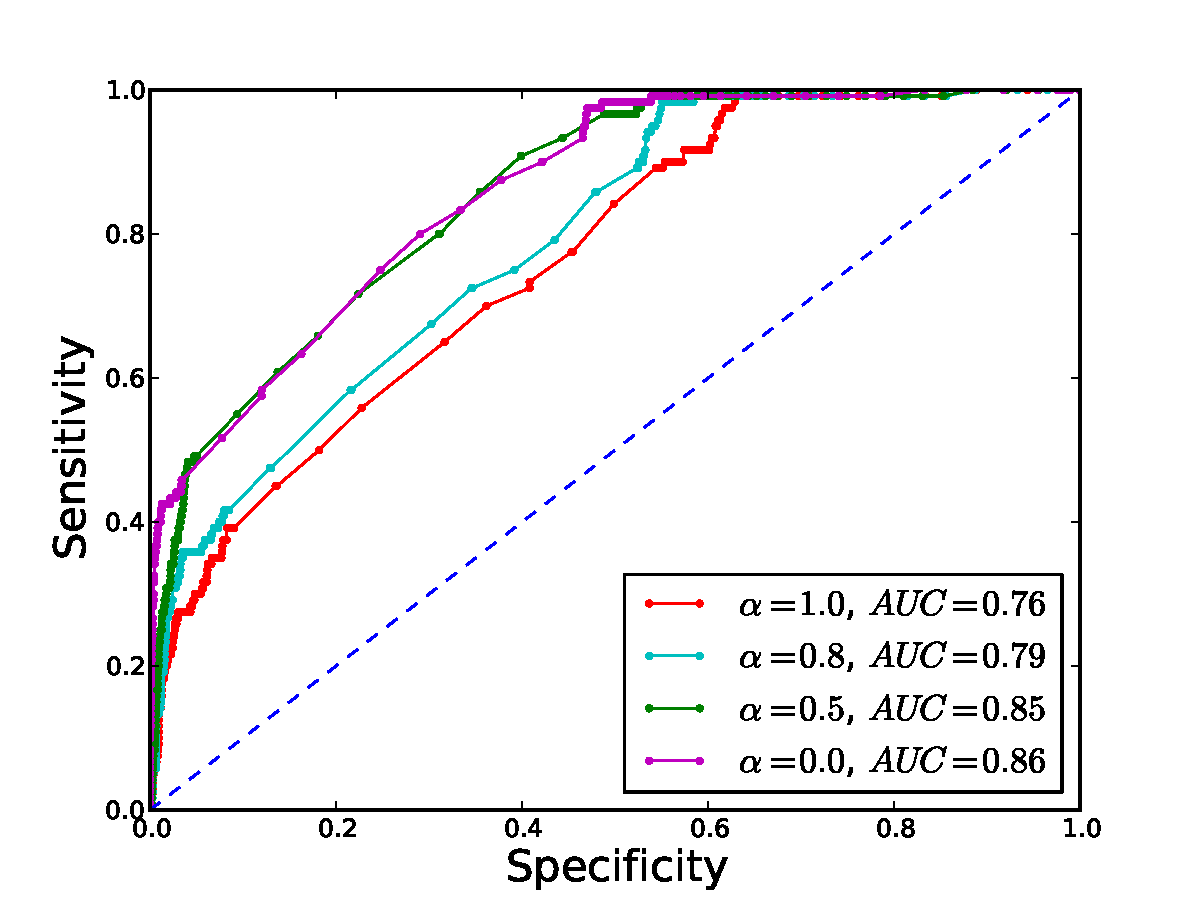
\includegraphics[width=1.2\textwidth]{figures/ROC_24.pdf}
%\caption{24 mutations}
%\label{fig:ROC24mut}
%\end{subfigure}
\caption{Performance of error-correction. Subfigures show accuracy with under-estimated error rates (6 mutations), exact estimates (12 mutations) and over estimates 
(24 mutations). We also analyze the impact of the parameter $\alpha$ distributing the weights of stacking pair energies vs isostericity scores and use values 
ranging of $\alpha=\{0,0.5,0.8,1.0\}$. The AUC is indicated in the legend of the figures. Each individual ROC curve represent the average performance over the 10 experiments.}
\label{fig:ROCall}\SpaceCheating
\end{figure}

Our data demonstrates that our algorithm shows interesting potential for error-correction applications. First, the AUC values (up to $0.86$) indicate that a
signal has been successfully extracted. This result has been achieved with errors in loop regions (i.e. without base pairing information) and thus suggests
that correction rates in structured regions (i.e. base paired regions) could be even higher. Next, the optimal values of $\alpha$ tend to be close to $0.0$. This 
finding suggests that, at this point, the information issued from the consideration of stacking energies is currently modest. However, specific examples showed improved performance
using this energy term. Further studies must be conducted to understand how to make the best use of it. Finally, our algorithm seems robust to the number of
presumed mutations. Indeed, good AUC values are achieved even with conservative estimates for the number of errors (c.f.~50\% of the errors, leading to 
Fig.~\ref{fig:ROCall}(a)), as well as with large  values (cf~200\% of the errors  in Fig.~\ref{fig:ROCall}(c)). It is worth noting that scoring schemes giving a larger weight on
the isostericity scores (i.e. for low $\alpha$ values) seem more robust to under- and over-estimating the number of errors.

\subsection{Correcting Illumina sequencing errors in 16s rRNAs}
\label{sec:16S}
\TODOTous{Describe and present results????}

To complete our benchmark, we turned to the small subunit ribosomal RNA in bacteriae, a molecule which is of particular interest  in metagenomics and phylogenetics. Our aim was to get as close as possible to a pyrosequencing context, in which reads are produced non-uniformly by an Illumina sequencer, impacting the distribution of errors in the sequence. 
We chose this setting both because of the popularity of Illumina sequencing in metagenomics, and since the underlying sequencing technique only considers base substitutions (no insertions), the only type of errors currently detected by \RNApyro.
To that purpose, we used simulated Illumina reads, mapped the reads back to a reference alignment, and run \RNApyro on a consensus sequence derived from the mapped reads, estimating the maximal amount of mutations from both the length of the sequence and the sequencing depth.


We gathered the seed sequences of the bacterial multiple sequence alignment (MSA) retrieved from the RFAM Database 11.0 (Rfam id: RF00177)~\cite{gardner2011rfam}. This alignment is composed of 93 sequences, whose length varies between 1461 and 1568 nucleotides, and has an average pairwise sequence identity of $69\%$. We used the pseudoknot-free version of the consensus secondary structure. A secondary structure for a specific reference sequence was obtained by simply mapping the structure back to sequence, i.e. by removing any base-pair having at least one partner involved in a gapped position. For similar reasons, we locally excluded from our calculation of the isostericity contribution for a given base-pair, described in Section~\ref{sec:model}, any sequence featuring at least a gap on the corresponding positions.

To simulate sequencing errors, we used the next-generation sequencing read simulator 
{\tt ART}~\cite{huang2012art}. The \emph{Illumina technology} setting was chosen as the main error mode, generating reads of $75~\text{bps}$, featuring mostly base substitution errors. Reads were mapped back to the original sequence, and a consensus sequence was determined, from the sequencing output, by a simple majority vote in the case of multiple coverage. Uncovered regions were simply generated at random. The average  rate of errors observed in the final consensus sequence was empirically estimated to represent $2.4\%$, $0.9\%$ and $0.6\%$ of the reference sequence, for prescribed sequencing coverages of $5$, $10$ and $15$ fold respectively.

As in Section~\ref{sec:5S}, we evaluated the predictive power of \RNApyro-computed mutational profiles using a leave-one-out strategy. We picked a sequence at random from the MSA, sequenced/mutated it as above, and run \RNApyro to establish its mutational profile. In this execution, we used values of $\beta=15$ and $\alpha\in [0, 0.5, 0.8, 1.0]$, and set the presumed number of mutations to twice the average error rate made by {\tt ART}, i.e. $4.8\%$, $1.8\%$ and $1.2\%$ for fold coverages of $5$, $10$ and $15$ respectively.
We repeated the whole procedure $12$/$10$/$14$ times for the $5$/$10$/$15-$fold coverage. 
We evaluated the predictive power of the profile by a computing a joint ROC curve for each value of $\alpha$, and each coverage, as described in Section~\ref{sec:5S}. Figure~\ref{fig:16s_all} shows the ROC curves, computed over all positions, while Figure~\ref{fig:16s_bp} only focuses on positions that are paired in the consensus secondary structure.



 



 \begin{figure}
\centering
\begin{subfigure}{.33\textwidth}
  \centering
  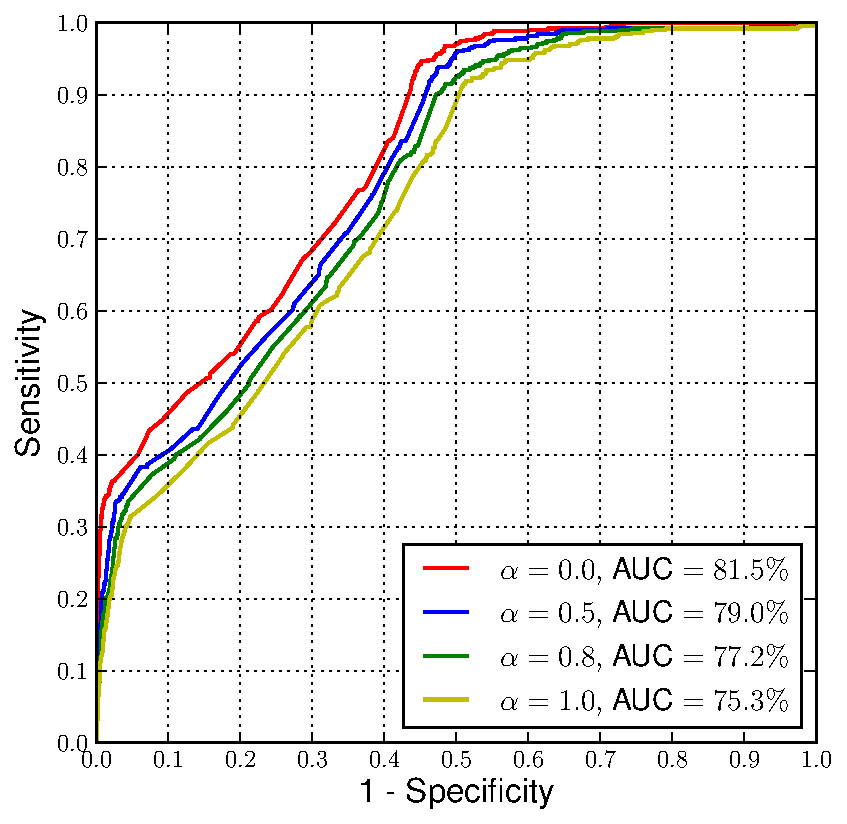
\includegraphics[width=\linewidth]{figures/5fold-a}
  \caption{$5-$fold coverage}
\end{subfigure}%
\begin{subfigure}{.33\textwidth}
  \centering
  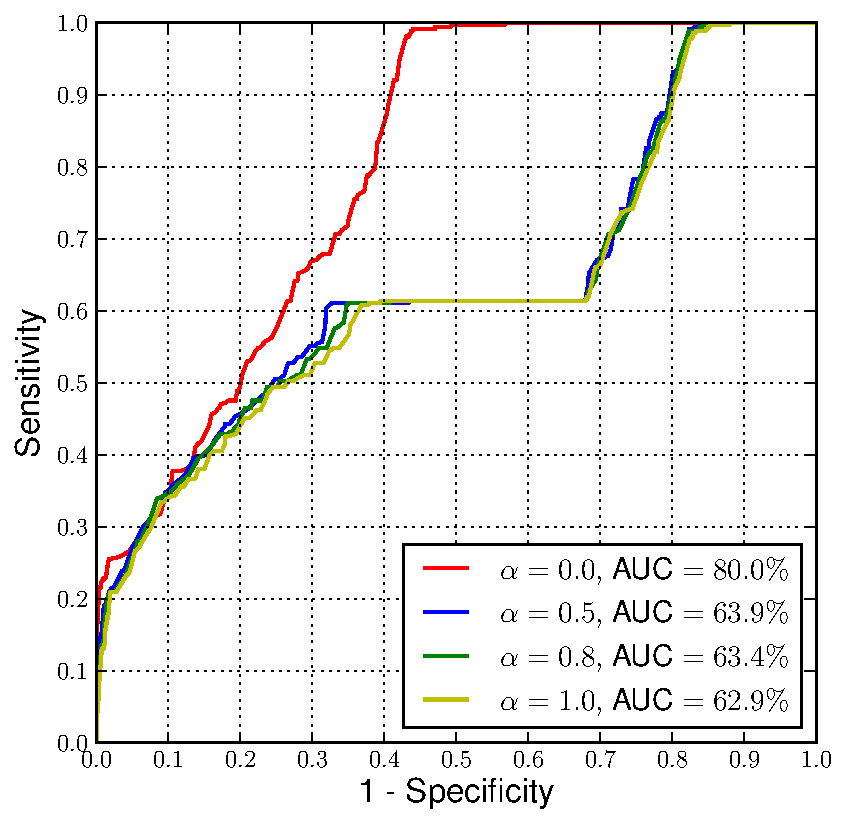
\includegraphics[width=\linewidth]{figures/10fold-a}
    \caption{$10-$fold coverage}
\end{subfigure}
\begin{subfigure}{.33\textwidth}
  \centering
  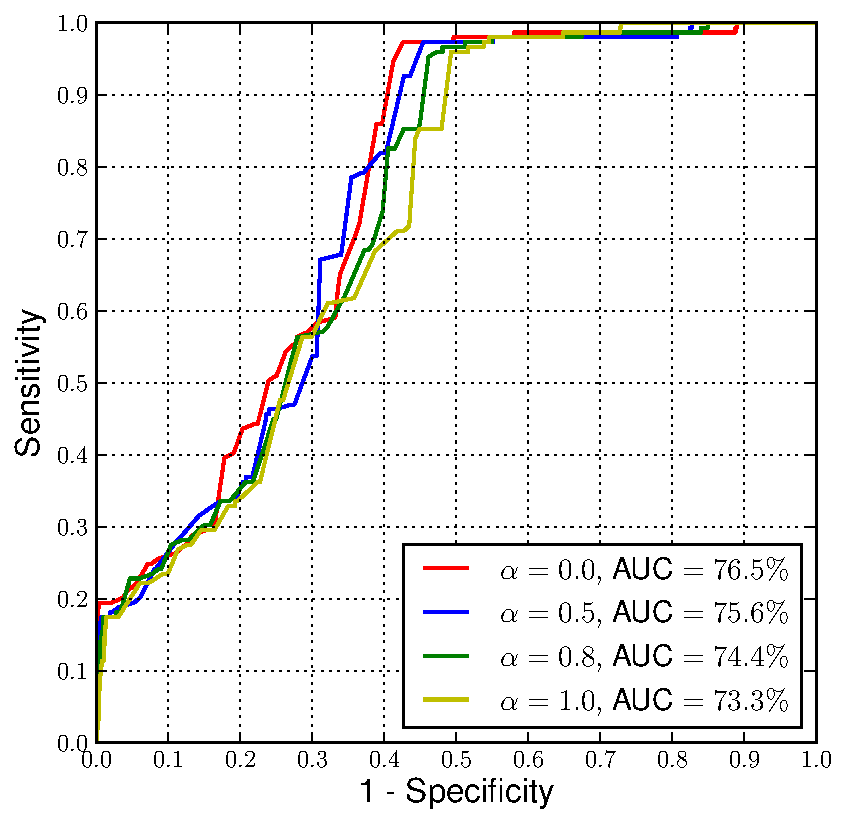
\includegraphics[width=\linewidth]{figures/15fold-a}
    \caption{$15-$fold coverage}
\end{subfigure}
\caption{Performance of error-correction over all positions. Subfigures show accuracy when
ART fold parameter is set to 5, 10 and $15-$fold coverage. We also analyze the impact of the parameter $\alpha$ distributing the weights of stacking pair energies vs isostericity scores and use values ranging of $\alpha = \{0, 0.5, 0.8, 1.0\}$. The AUC is indicated in the legend of the figures. Each individual ROC curve represent the average performance over at least 10 experiments.}

\label{fig:16s_all}
\end{figure}

 \begin{figure}
\centering
\begin{subfigure}{.33\textwidth}
  \centering
  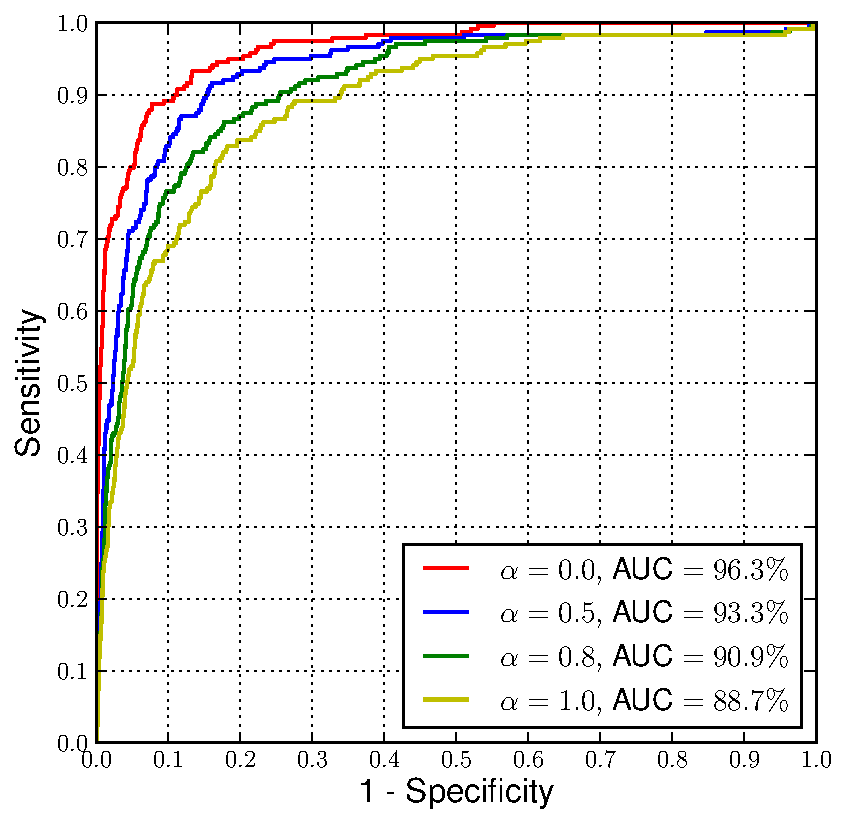
\includegraphics[width=\linewidth]{figures/5fold-b}
  \caption{$5-$fold coverage}
\end{subfigure}%
\begin{subfigure}{.33\textwidth}
  \centering
  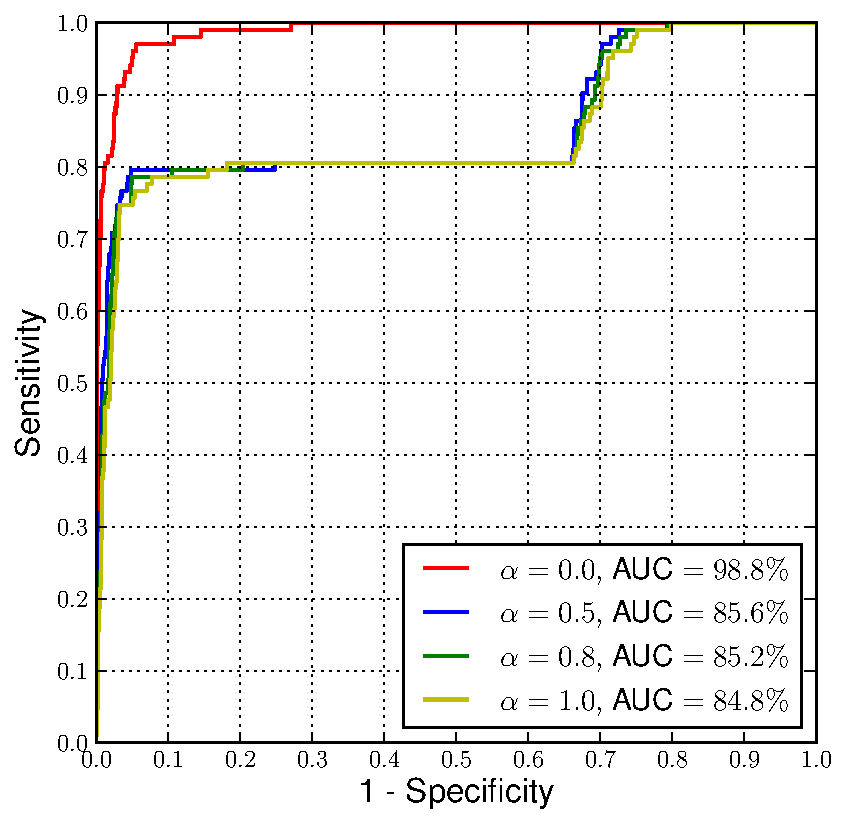
\includegraphics[width=\linewidth]{figures/10fold-b}
    \caption{$10-$fold coverage}
\end{subfigure}
\begin{subfigure}{.33\textwidth}
  \centering
  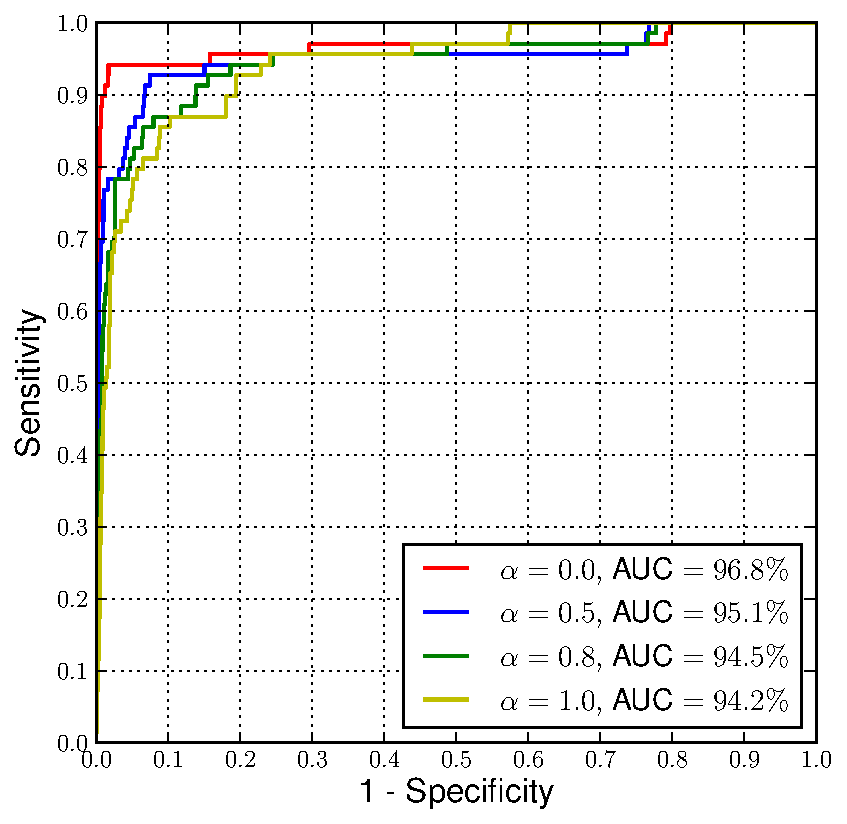
\includegraphics[width=\linewidth]{figures/15fold-b}
    \caption{$15-$fold coverage}
\end{subfigure}
\caption{Performance of error-correction over structured positions (i.e. inside a base pair). Subfigures show accuracy when
ART fold parameter is set to 5, 10 and $15-$fold coverage. We also analyze the impact of the parameter $\alpha$ distributing the weights of stacking pair energies vs isostericity scores and use values ranging of $\alpha = \{0, 0.5, 0.8, 1.0\}$. The AUC is indicated in the legend of the figures. Each individual ROC curve represent the average performance over at least 10 experiments.}
\label{fig:16s_bp}
\end{figure}

Our data demonstrates that even on long sequences our algorithm shows interesting potential for 
error-correction applications. First, the AUC values (up to 0.81) when looking at all positions, 
in Fig.~\ref{fig:16s_all},  indicate that a signal has been successfully extracted. When restraining
to structured regions (i.e. base paired regions) we obtain AUC values up to 0.998.  Since 
contributions to the energy and isostericity only arise from structured regions, this was an expected result.

An interesting feature is that best results are almost always when $\alpha=0$, i.e. all the contribution
comes from the isostericity. A notable exception is when the number of mutation is underestimated, 
in that case best performances were observed for non-null values of $\alpha$.

Another observation is when we look at all positions as in Fig.~\ref{fig:16s_all}. The first $20\%$ to $30\%$ of sensitivity are obtained almost without any errors and correspond to the nucleotides in 
structured regions. The rest of the predictions are done on un-paired nucleotides.

